\documentclass[]{thesis}


\DeclareAcronym{SAT}{
  short=SAT,
  long=boolean satisfiability problem,
}

\DeclareAcronym{DL}{
  short=DL,
  long=deep learning,
}

\DeclareAcronym{ML}{
  short=DL,
  long=machine learning,
}

\DeclareAcronym{GNN}{
  short=GNN,
  long=graph neural network,
}

\DeclareAcronym{MUS}{
  short=MUS,
  long=minimal unsatisfiable subset,
  short-plural=es,
}

\DeclareAcronym{PGE}{
  short=PGExplainer,
  long=parameterized explainer for graph neural networks,
}

\DeclareAcronym{MLP}{
  short=MLP,
  long=multilayer perceptron,
}

\DeclareAcronym{GCN}{
  short=GCN,
  long=graph convolutional network,
}

\DeclareAcronym{CNN}{
  short=GCN,
  long=convolutional neural network,
}

\DeclareAcronym{MPNN}{
  short=MPNN,
  long=message passing neural network,
}

\DeclareAcronym{CNF}{
  short=CNF,
  long=conjunctive normal form,
}

\DeclareAcronym{LCG}{
  short=LCG,
  long=literal-clause graph,
}

\DeclareAcronym{ROC-AUC}{
  short=ROC-AUC,
  alt = AUROC,
  long=area under the receiver operating characteristic curve,
}

\DeclareAcronym{ROC}{
  short=ROC,
  long=receiver operating characteristic,
}

\DeclareAcronym{AUC}{
  short=AUC,
  long=area under the curve,
}

\DeclareAcronym{GT}{
  short=GT,
  long=ground truth,
}

\DeclareAcronym{BA}{
  short=BA,
  long=Barabási-Albert,
}

\DeclareAcronym{TM}{
  short=TM,
  long=target model,
}


\begin{document}

    \definecolor{codegreen}{rgb}{0,0.6,0}
    \definecolor{codegray}{rgb}{0.5,0.5,0.5}
    \definecolor{codepurple}{rgb}{0.58,0,0.82}
    \definecolor{backcolour}{rgb}{0.95,0.95,0.92}


    \lstdefinestyle{mystyle}{
        backgroundcolor=\color{backcolour},   
        commentstyle=\color{codegreen},
        keywordstyle=\color{magenta},
        numberstyle=\tiny\color{codegray},
        stringstyle=\color{codepurple},
        basicstyle=\ttfamily\footnotesize,
        breakatwhitespace=false,         
        breaklines=true,                 
        captionpos=b,                    
        keepspaces=true,                 
        numbers=left,                    
        numbersep=5pt,                  
        showspaces=false,                
        showstringspaces=false,
        showtabs=false,                  
        tabsize=2
    }

    \lstset{style=mystyle}

    \pagenumbering{roman}
    \begin{titlepage}
    \begin{center}
        \begin{minipage}[t]{\textwidth}
            \raggedleft
            \includegraphics[width=0.35\textwidth]{img/tud-logo.pdf}
        \end{minipage}
    
        \vspace{3cm}
            
        \Huge
        \textbf{Providing Bipartite GNN Explanations with PGExplainer}
            
        \vspace{1.5cm}
            
        \LARGE
        \textbf{Tristan Marten Lewin Schulz}
            
        \vspace{1.5cm}
          
        \Large
        Bachelor of Science\\
        May 19, 2025\\
    \end{center}

    \vfill

    \noindent
    \begin{minipage}[t]{0.5\textwidth}
        \raggedright
        \Large
        Supervisors:\\
        Prof. Dr. Stefan Harmeling\\
        Lukas Schneider\\
    \end{minipage}
    \hfill
    \begin{minipage}[t]{0.5\textwidth}
        \raggedleft
        \Large
        Artificial Intelligence (VIII)\\
        Department of Computer Science\\
        TU Dortmund University\\
    \end{minipage}
\end{titlepage}

    \cleardoublepage

    \phantomsection
    \addcontentsline{toc}{chapter}{Abstract}
    \chapter*{Abstract}

%Context/Background: Why is this topic and this research important?
%Objective: What questions are you trying to answer in your research?
%Methods/Design: What are the basic details of your research? In general, how did you go %about answering the research questions? 
%Results: What answers did you find? Were there any other observations?
%Conclusion/Takeaways: Were your results expected? Is more research needed?


The recent advances in \ac{DL} have lead to \ac{ML} approaches for solving the \ac{SAT}, commonly represented as a bipartite graph problem, with NeuroSAT being a prominent example utilizing a \ac{GNN}. However, models like these often suffer from a lack of natural proofs or explanations of their predictions, hindering the trustworthiness as well as practical cross-domain applicability. In this work, we explore a method that provides instance explanations with a global view of the GNN, thus seeking to generally explain a model's predictions. We reimplement the \ac{PGE} using PyTorch Geometric, testing its generalizability in the inductive setting and extending it to the domain of NeuroSAT.

While our replication showed that the framework succeeds in generating inductive explanations for structurally similar node instances, it struggles with generalizing these across different node instances of a motif. At the same time, general explanations for graph instances showed promising results. To apply the PGExplainer on NeuroSAT and generate explanations for SAT instances, we interpret unsatisfiable SAT instances using \acp{MUS} - small unsatisfiable cores - as \ac{GT}. Though we were unable to generate favorable explanations that consistently align with these, our findings indicate potential measures for future work and highlight the need for more robust and generalizable methods. 
    \cleardoublepage

    % USE THIS TO HIDE SUBSECTIONS IN TOC
    \setcounter{tocdepth}{1}
    \tableofcontents
    \cleardoublepage

    \cleardoublepage
    \phantomsection
    \addcontentsline{toc}{chapter}{List of Figures}
    \listoffigures

    \cleardoublepage
    \phantomsection
    \addcontentsline{toc}{chapter}{List of Tables}
    \listoftables

    \cleardoublepage
    \phantomsection
    \addcontentsline{toc}{chapter}{List of Variables}
    \chapter*{List of variables}

\begin{description}
    \item[$X$] A discrete random variable
    \item[$p(x)$] The probability mass function of $X$
    \item[$H(X)$] The entropy of the random variable $X$
    \item[$\mathbf{x} \in \mathbb{R}^d$] A feature vector of $d$ features
    \item[$\mathbf{w} \in \mathbb{R}^d$] A weight vector of $d$ weights
    \item[$\mathbf{c} \in \mathbb{R}^m$] A vector of $m$ bias terms
    \item[$\mathbf{W} \in \mathbb{R}^m\times d$] A weight matrix of $m$ units and $d$ features
    \item[$\boldsymbol{\theta}$] A set of model parameters
    \item[$\mathbf{h} \in \mathbb{R}^d$] A vector of $d$ hidden unit activations or hidden features
    \item[$b \in \mathbb{R}$] A bias scalar 
    \item[$\Omega(\boldsymbol{\theta})$] A regularization term (e.g., an $L_2$-norm penalty on the parameters)
    \item[$\mathcal{B} \in \mathbb{R}^{m\times d}$] A minibatch design matrix of activations
    \item[$\mathcal{B}' \in \mathbb{R}^{m\times d}$] The normalized version of $B$
    \item[$\boldsymbol{\mu} \in \mathbb{R}^m$] A vector containing the mean of each unit
    \item[$\boldsymbol{\sigma} \in \mathbb{R}^m$] A vector containing the standard deviation of each unit
    
    \item[$s$] The expectation of a function $f(x)$ under the distribution $p(x)$
    \item[$\hat{s}_N$] The Monte Carlo estimate of the expectation, based on $N$ samples.
  \end{description}

    \cleardoublepage
    \phantomsection
    \addcontentsline{toc}{chapter}{List of Acronyms}
    \acsetup{list/name = {List of Acronyms}}
    \printacronyms

    \cleardoublepage
    \pagenumbering{arabic}
    \chapter{Introduction}
\label{ch:Introduction}

Solvers for \ac{SAT} are one of many applications that have seen progress through the development of \ac{DL} in recent years. NeuroSAT \cite{selsam2018learning} is one exemplary framework that combines \ac{ML} with SAT solving. Since SAT instances can naturally be represented as bipartite graphs, \acp{GNN} or \acp{MPNN} are a logical choice for solving this task. However, NeuroSAT lacks the ability of providing proofs to its predictions of unsatisfiability, which are required to compete with state-of-the-art SAT solvers \cite{audemard2009predicting}, \cite{een2003extensible}. This is one example of the general need for explanations that establish trust in the predictions of GNNs \cite{guo2023machine}, \cite{ribeiro2016should}. \bigskip

Several approaches have been developed to explain the predictions made by deep graph models. One perturbation-based method is the \ac{PGE} \cite{luo2020parameterized} whose explanations provide a global, generalizable understanding of the underlying trained GNN. It learns approximated discrete edge masks from GNN representations of input graphs to explain instance predictions. Since the masks are sampled from a mask predictor shared across all edges in the dataset, it is able to provide explanations with a global view of the model \cite{luo2020parameterized}, \cite{yuan2022explainability}. Moreover, this allows for the application in an inductive setting, where unexplained test instances can be explained without being used during training, as opposed to the collective setting used in previous works.\bigskip

We will start this work by introducing the theoretical background, including the concepts of GNNs and explainability in GNNs \cite{yuan2022explainability}. After explaining the main concepts of PGExplainer \cite{luo2020parameterized} we re-implement the model, as well as the underlying GNNs, using PyTorch Geometric \cite{Fey/Lenssen/2019} rather than the originally used library TensorFlow \cite{tensorflow2015-whitepaper}. Additionally, we introduce slight changes to the GNN design in regard to bipartite graphs to verify if the explainer, as claimed by the authors, is invariant to changes in model architecture. The generated explanations are evaluated using both qualitative and quantitative metrics, which we further use to optimize the model. We will then compare our results to the baseline of the original paper, as well as a present replication study, while focusing on the application in the inductive setting. \cite{holdijk2021re}. \bigskip

After a successful replication of the baseline experiments we aim to apply the explainer method to NeuroSAT. In doing so, we aim to learn and generate general, retrospective bipartite explanations of unsatisfiable instances that support the predictions of NeuroSAT. Since we require \acp{GT} to evaluate the accuracy of explanations, we propose treating \acp{MUS} - small unsatisfiable cores - of the instances as expected \ac{GT}. We justify this with the fact that unsatisfiable SAT instances can be "reduced" to MUSes by perturbing the edges outside the subset, which represent appearances of literals in clauses not included in the subset. Ultimately, our goal is testing whether the explanations provided for NeuroSAT align with "human-understandable" principles, specifically the appointed MUS \ac{GT}.
    \chapter{Background}
\label{ch:Background}
In this chapter we define the necessary background for understanding PGExplainer as well as the follow-up work regarding its application on the Boolean Satisfiability Problem (SAT).

\section{TODO Deep learning}
In this chapter we introduce Deep Learning (DL) in the context of Machine Learning (ML) and their concepts required for this work. \\
What is machine learning? What is Deep learning? \\
Types of tasks in machine learning; Classification task in our case; \\
Supervised vs unsupervised learning; \\
All definitions in this chapter follow Goodfellow et al.\cite{Goodfellow-et-al-2016}. 

\subsection{Deep Feedforward Networks/MLP}
A classical deep learning model is the multilayer perceptron (MLP) with the general goal of approximating a function $f^*$. In the case of classification we could define a function $y = f^*(x)$ that maps an input $x$ to a label $y$. The MLP then defines the mapping $y = f(x;\Theta)$ and learns the value of the parameters $\Theta$ that best approximate the function. These models are also referred to as feedforward neural networks, as they process information from $x$, through the intermediate computations that define $f$, to the output $y$ without feedback connections that would feed outputs back to itself. The name network is derived from their representation as a composition of multiple different functions, that are described by a directed acyclic graph. An example network is $f(x) = f^{(3)}(f^{(2)}(f^{(1)}(x)))$ that consists of first layer $f^{(1)}$, second layer $f^{(2)}$ and output layer $f^{(3)}$. The length of this chain of functions is called depth and origin of the term "deep learning". The approximation is achieved by training our network with training data, that consists of approximated examples of $f^*(x)$ at different points in the training and labels $y\approx f^*(x)$. These training examples dictate the output layer to generate a value close to $y$ for each $x$. The learning algorithm then learns to utilize the other hidden layers, without specified behaviors, to achieve the best approximation. It is to note that the hidden layers are vector-valued, with each vector element, referred to as unit, loosely taking the role of a neuron in neuroscience.
\subsection{Gradient descent}

\subsection{Computational graph}

\subsection{Backpropagation}

\subsection{Regularization}

\subsection{Batchnorm, LayerNorm, ...}

\subsection{TODO Weight Matrix somewhere}

\subsection{Monte Carlo Sampling}
Goodfellow et al.\cite{Goodfellow-et-al-2016}[p.590] TODO: EXPLANATION \\
Let 
\begin{equation}
    s = \sum_x p(x)f(x)=E_p[f(x)]
\end{equation}
be the sum to estimate with $p$ being a probability distribution over a random variable $x$. Then $s$ can be approximated by drawing $n$ samples from $p$ and constructing the empirical average 
\begin{equation}
    \hat{s}_n=\frac{1}{n}\sum_{i=1}^n f(x^{(i)}).
\end{equation}


\section{Graph Theory}
These definitions will loosely follow Liu et al.\cite{Liu2020}. A graph is a data structure consisting of a set of nodes that are connected via edges, modeling objects and their relationships. It can be represented as $G=(V,E)$ with $V=\{v_1,v_2...v_n\}$ being the set of $n$ nodes, and $E \in V \times V$ the set of edges. An edge $e=(u,v)$ connects nodes $u$ and $v$, making them neighbours. Edges are either directed or undirected and lead to directed or undirected graphs if exclusively present. The degree of a node $v$ is the number of edges connected to $v$ and denoted by $d(v)$. $G$ can be described by an adjacency matrix $A \in \mathbb{R}^{n \times n}$, where
\begin{equation*}
    A_{ij}=\begin{cases}
        1 & \text{if } \{v_i,v_j\}\in E \text{ and } i \neq j, \\
        0 & \text{otherwise.}
    \end{cases}
\end{equation*}
If $G$ is an undirected Graph the adjacency matrix will be symmetrical. \\
Alternatively an undirected graph $ G=(V, E)$ with $n$ nodes and $m$ edges can be represented as an incidence matrix $M \in \mathbb{R}^{n \times m}$, where
\begin{equation*}
    M_{ij}=\begin{cases}
        1 & \text{if } \exists k \text{ s.t. } e_j = \{v_j, v_k\} \\
        0 & \text{otherwise.}
    \end{cases}
\end{equation*}
We adopt the conventions from Diestel\cite{Diestel2017} to refer to the node and edges set of any graph $G$ with $V(G)$ and $E(G)$ respectively, regardless of the actual names of the sets, as well as a referring to $G$ with node set $V$ as $G$ on $V$. $G$ is called a subgraph of another graph $G'=(V',E')$ if $V(G) \subseteq V(G')$ and $E(G) \subseteq E(G')$. This is denoted as $H \subseteq G$. The number of nodes in a graph $|V|$ is its order and the number of edges $|E|$ is its size.
We additionally define bipartite graphs according to Asratian et al.\cite{asratian1998}: A graph $G$ is bipartite if the set of nodes $V$ can be partitioned into two sets $V_1$ and $V_2$ so that no two nodes from the same set are adjacent. The sets $V_1$ and $V_2$ are called colour classes and $(V_1, V_2)$ is a bipartition of $G$. This means that if a graph is bipartite all nodes in $V$ can be coloured by at most two colours so that no two adjacent nodes share the same colour.\\
TODO: EDGE WEIGHTS, K-hop/computational graph?
\begin{figure}[h]
    \centering
    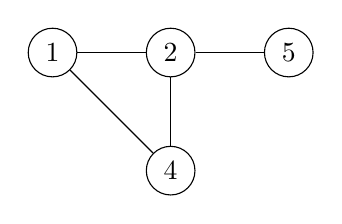
\begin{tikzpicture}[node distance=1.5cm, every node/.style={draw, circle}]
        % Define Nodes
        \node (1) {1};
        \node (2) [right of=1] {2};
        \node (4) [below of=2] {4};
        \node (5) [right of=2] {5};
        
        % Draw Edges
        \draw (1) -- (2);
        \draw (2) -- (4);
        \draw (1) -- (4);
        \draw (2) -- (5);
    \end{tikzpicture}
    \caption{A simple undirected graph $G$ with $V=\{1,...,5\}$ and $E=\{\{1,2\},\{2,4\},\{1,4\},\{2,5\}\}$}
    \label{fig:graph-example}
\end{figure}

\subsection{TODO Graph generation/Graph Generative Model/Random Graphs}
Erdos-Renyi model first model of random graphs, but slightly different from Gilbert. \bigskip

Gilbert\cite{} describes the process of generating a random graph of order $N$ by assigning a common probability to exist in the graph to each potential edge between two nodes. Note that these random selections are made independently of each other, effectively drawing from a Bernoulli distribution. \\
by performing independent experiments for each potential edge between two nodes of the graph. Since these experiments share a common probability, the process can be described as drawing from a Bernoulli distribution. \\
A random graph is further described by Diestel\cite{} as follows. Let $V = \{0,...,n-1\}$ be a fixed set of $n$ elements. Our goal is to define the set $\mathcal{G}$ of all graphs on $V$ as a probability space, which allows us to ask whether a Graph $G \in \mathcal{G}$ has a certain property. To generate our random graph we then decide from some random experiment whether $e$ shall be an edge of $G$ for each potential $e \in V \times V$. The probability of success - accepting $e$ as edge in $G$ - is defined as $p \in [0,1]$ for each experiment. TODO: Rewrite the accepting part. This leads to the probability of $G$ being a particualar graph $G_0$ on $V$ with e.g. $m$ edges being equal to $p^m q^{\binom{n}{2}-m}$ with $q:=1-p$. It follows our desired probability space $\mathcal{G}=(n,p)$ as the product space
$$\Omega := \prod_{e \in [V]^2} \Omega_e$$ with $\Omega_e := \{0_e,1_e\}$, $\mathbb{P}_e(\{1_e\}) := p$ and $\mathbb{P}_e(\{0_e\}) := q$.
$$E(G) = \{e | \omega(e) = 1_e\}$$
G is called a random graph on V with egde probability p. \bigskip

INSTEAD: Gilberts idea also assigns the same probability across all edges, so probably best to explain the general idea as presented in Diestel. Then explain the difference in PGE? PGEs appraoch mainly inspired by probabilistic graphical model/bayesian networks. Gilbert model mainly baseline for probabilistic graphs. PGExplainer mainly inspired by Gilbert, but "required" concept is PGM.

\section{Information Theory}
To fully understand the learning objective of PGExplainer it is necessary to define the concepts of entropy and mutual information. We follow the definitions by Cover et al.\cite{Cover2005}[p.13].

\subsection{Entropy}
TODO: REVISE THIS. Probably best to define with general expactation, for continous and discrete, according to Goodfellow. Derive conditional entropy for general case. Only apply discrete case where needed? (cross entropy in PGE) \bigskip

Entropy is used to describe the uncertainty of a random variable. It measures the amount of information required on average to describe a random variable. Let $X$ be a discrete random variable with alphabet $\mathcal{X}$ and probability mass function $p(x)=Pr\{X=x\}$ for $x\in X$.
The entropy $H(X)$, also written as $H(p)$, is defined as
\begin{equation}
    H(X) = -\sum_{x \in \mathcal{X}} p(x) \log p(x).
\end{equation}
TODO: WE USE NATURAL LOGARITHM IN CODE! The log is to the base $e$ and entropy is measured in nats. TODO: DEFINE EDGE CASES log 0 TODO: TOO MUTCH + SOURCE? A simple example is tossing two coins: There are four possible outcomes $\mathcal{X}=\{00,10,01,11\}$, 0 for heads and 1 for tails, each with a probability $p=0,25$. The resulting entropy $H(X)=2$ represents that two bits of information can be stored this way. \bigskip

%TODO: DIFFER MORE CLEARLY FROM CROSS? \\
%Analogously we define the joint entropy $H(X,Y)$ of a pair of discrete random variables $(X,Y)$ with a joint distribution $p(x,y)$ as follows:
%\begin{equation}
%    H(X,Y)=-\sum_{x \in \mathcal{X}} \sum_{y \in \mathcal{Y}} p(x,y) \log p(x,y).
%\end{equation}
The conditional entropy of $Y$ given $X$ is defined as the expected value of the entropies of the conditional distributions, averaged over the conditioning random variable. If $(X,Y) \sim p(x,y)$ for a pair of discrete random variables $(X,Y)$ with joint distribution $p(x,y)$, the conditional entropy is defined as \\
\begin{align}
    H(Y|X)&= -\sum_{x \in \mathcal{X}} p(x) H(Y|X=x) \\
    &= - \sum_{x \in \mathcal{X}} \sum_{y \in \mathcal{Y}}p(x,y) \log p(y|x) \\
    &= -E \log p(Y|X) \text{ with E = Expectation}.
\end{align}

Elements of Information Theory: equation 2.26 describes KL distance/relative entropy \bigskip

The following definitions loosely follow Goodfellow et al.\cite{Goodfellow-et-al-2016}[p.74].
The relative entropy is a measure of the distance between two distributions.
"measure how different these two distributions are" \cite{Goodfellow-et-al-2016}
"In the case of discrete variables, it is the extra amount of information needed to send a message containing symbols drawn from probability distribution P, when we use a code that was designed to minimize the length of messages drawn from probability distribution Q."
"The KL divergence is 0 if and only if P and Q are the same distribution in the case of discrete variables"
non symmetrical.
"When computing many of these quantities, it is common to encounter expressions of the form 0 log 0. By convention, in the context of information theory, we treat these expressions as limx→0 x log x = 0. \\
We define the KL divergence or relative entropy between two probability distributions $P, Q$ as
\begin{equation}
    D_{KL}(P||Q) = \sum_{x \in \mathcal{X}} P(x)\log \frac{P(x)}{Q(x)}
\end{equation}

The cross entropy is closely related to KL distance and therefore defined as
\begin{align}
    H(P,Q) &= -\mathbb{E}_{x\sim P}\log Q(x) \\
    &= H(P) + D_{KL}(P||Q)
\end{align}

We derive for the discrete case with mass probability functions $p, q$ defined on the same support $\mathcal{X}$:
\begin{align}
    H(p,q) = H(p) + D_{KL}(p||q) &= -\sum_{x \in \mathcal{X}} p(x) \log p(x) + \sum_{x \in \mathcal{X}} p(x)\log \frac{p(x)}{q(x)} \\
    &= -\sum_{x \in \mathcal{X}} p(x) \log p(x) + \sum_{x \in \mathcal{X}} p(x) \log p(x) -\sum_{x \in \mathcal{X}} p(x) \log q(x) \\
    &= -\sum_{x \in \mathcal{X}} p(x) \log q(x)
\end{align}

The approach in PGExplainer is a common approach in ML for simplifying objectives? FIND LITERATURE THAT EXPLAINS APPROXIMATION OF COND. ENTROPY WITH CROSS ENTROPY. Explanation as simple as one formula for one graph variable example, cross entropy applied to whole distribution? \bigskip

"We can modify the conditional entropy objective in Equation 4 with a cross entropy objective between the label class and the model prediction" (GNNExplainer)

\subsection{Mutual Information}
Another closely related concept is mutual information (see Cover et al.\cite{Cover2005}[p.19]). It measures the amount of information that one random variable contains about another or the reduction in uncertainty of said variable due to knowing the other.
Let $X$ and $Y$ be two random variables with the joint probability mass function $p(x,y)$ and marginal probability mass functions $p(x)$ and $p(y)$. Mutual information $I(X;Y)$ is the relative entropy between the joint distribution and the product distribution $p(x)p(y)$: 
\begin{align}
    I(X;Y)&=\sum_{x \in \mathcal{X}}\sum_{y \in \mathcal{Y}} p(x,y)\log \frac{p(x,y)}{p(x)p(y)} \\
    &= H(X) - H(X|Y)
\end{align}

\section{TODO Graph Neural Networks}

The following definitions will loosely follow book/... (reference).
JEDE Variable einmal erklärt! Einheitliche Variablen aus meiner Sicht

Graph Neural Networks(GNNs)\cite{4700287} are a deep learning-based approach that operates on graphs, a data structure consisting of nodes and edges, representing objects and their relationships. Due to their unique non-Euclidean property, they find usage in classification, link prediction, and clustering tasks. Their high interpretability and strong performance have led to GNNs becoming a commonly employed method in graph analysis. They combine the key features of convolutional neural networks\cite{726791}, such as local connection, shared weights, and multi-layer usage, with the concept of graph embeddings\cite{cai2018comprehensive} to leverage the power of feature extraction and representation as low-dimensional vectors for graphs\cite{Liu2020}. \\
- difference node classification, graph classification (Scarselli) \\
- data preprocessed: mapping to simpler representation
- encode graph structure/topology to keep structural information
- directed/undirected?
- ...



\subsection{Convolutional Graph Neural Networks}
Explain? Used in architecture of downstream task, only slightly relevant

\section{Perturbation-based Explainability in GNNs}
Methods in deep learning have seen growth in performance in many tasks of artificial intelligence, including GNNs. However, the interpretability of these models is often limited due to their black-box design. Explainability methods aim to bypass this limitation by designing post-hoc techniques that provide insights into the decision-making process in the form of explanations. Such human-intelligible explanations are crucial for deploying models in real-world applications, especially when applied in interdisciplinary fields. There exist several different approaches for explaining predictions of deep graph models, that can be categorized into instance-level methods and model-level methods (see Yuan et al. \cite{yuan2022explainability}). Instance-level methods aim to explain each input-graph by identifying important input features for its prediction, leading to input-dependent explanations. These can further be grouped by their importance score calculation into gradients/feature-based, perturbation-based, decomposition methods and surrogate methods. Model-level methods, on the other hand, aim to explain GNNS without considering specific inputs, leading to input-independent, high-level explanations. \\
In this work we focus on the perturbation-based approach, more specifically the PGExplainer\cite{luo2020parameterized}, that aims to evaluate the change of prediction with respect to input perturbations. The intuition behind this is that when input information crucial to the prediction is kept, the new prediction should roughly align with the prediction from the original input. The general pipeline for different perturbation based approaches can be described as follows: First, the important features from the input graph are converted into a mask by our generation algorithm, depending on the explanation task at hand. These masks are applied to the input graph to highlight said features. Lastly, the masked graph is fed into the trained GNN to evaluate the mask and update the mask generation algorithm according to the similarity of the predictions. \\
It is important to distinguish between soft masks, discrete masks and approximated discrete masks. Soft masks take continuous values between $[0,1]$ which enables the graph algorithm to be updated via backpropagation. A downside of soft masks is that they suffer from the "introduced evidence" problem(see Dabkowski et al.\cite{ Dabkowski }). Any mask value that is non-zero or non-one may add new semantic meaning or noise to the input graph, since graph edges are by nature discrete. Discrete masks however always rely on non-differentiable operations, e.g. sampling. Thus, the approximated discrete masks utilize reparameterization tricks to avoid the "introduced evidence" problem while also enabling back-propagation. \\
Explanations can on the one hand be evaluated by visualizing the graph and considering the "human-comprehensibility". Since this requires a ground truth, is prone to the subjective understanding and is usually performed for a few random samples, it is important to apply stable evaluation metrics. TODO: One relevant accuracy metric for synthetic datasets with ground truths is the Area Under the Receiver Operating Characteristic Curve (ROC-AUC/AUC) (see Richardson et al.\cite{}). \\
\url{https://www.sciencedirect.com/science/article/pii/S2666389924001090?ref=pdf_download&fr=RR-2&rr=92785edbb946f803}
The Receiver Operating Characteristic (ROC) curve plots the False Positive Rate (FPR) on the x-axis against the True Positive Rate (TPR), across different classification thresholds. The area under the curve (AUC) is calculated for said curve, resulting in the ROC-AUC. It is important to note, that a value of $0.5$ equals random guessing, while a score of $1.0$ indicates perfect classification. \bigskip

TODO: \\
Explain TRP FPR?

Variation in perturbation approaches lie in: mask gen. alg., type of mask, objective function.

Differentiate between "interpretable" and "explainable"? Model itself provides human-understandable interpretations vs model still black box with explanations by post-hoc model.

- Other metric includes fidelity, results of taxonomy propose only using PGExplainer for Node Classification as it achieves low fidelity on Graph tasks

TODO: Perturbation pipeline?

\section{Boolean Satisfiability Problem}
We define the Boolean Satisfiability Problem (SAT) according to Guo et al.\cite{guo2023machine}[p.641]: \\
A Boolean formula is constructed from Boolean variables, that only evaluate to True (1) or False (0), and the three logic operators conjunction ($\wedge$), disjunction ($\vee$) and negation ($\neg$). SAT aims to evaluate whether there exists a variable assignment for a formula constructed of said parts so that it evaluates to True. If so, the formula is said to be satisfiable or unsatisfiable otherwise. Every propositional formula can be converted into an equivalent formula in conjunctive normal form (CNF), which consists of a conjunction of one or more clauses. These clauses must contain only disjunctions of at least one literal (a variable or its negation). In this work we consider only formulas in CNF, as NeuroSAT\cite{} assumes SAT problems to be in CNF. An example of a satisfiable formula in CNF over the set of variables $V=\{x_1,x_2\}$ is 
$$\psi(V) = (x_1) \land (\neg x_1 \lor x_2) \land (\neg x_2 \lor x_2)$$
with satisfying assignment $A:\{x_1 \mapsto 1, x_2 \mapsto 1\}$. Furthermore, SAT is $NP$-complete, meaning that if there exists a deterministic algorithm able to solve SAT in polynomial time, then such an algorithm exists for every $NP$ problem (see cook\cite{}). Current state of the art SAT solvers apply searching based methods such as Conflict Driven Clause Learning (GRASP marques silva)\cite{} or Stochastic Local Seach (TYPCIAL EXAMPLE WALKSAT: Local search strategies for satisfiability testing Profile image of Bart SelmanBart Selman)\cite{} with exponential worst-case complexity.

\subsection{Representation as Bipartite Graph}
SAT has extensively been studied in the form of graphs,
Guo et al. describe four different types of graph representations for CNF formulae with varying complexity and information compression. Since we want to minimize the loss of information for SAT we adapt the information-richest form of a literal-clause graph (LCG). 
A LCG is a bipartite graph that separates literals and clauses, with edges connecting literals to the clauses they appear in.
The resulting graph can formally be described by a biadjacency matrix $B$ of shape $l \times c$. \\
Let $A \in \mathbb{R}^{l+c \times l+c}$ be the adjacency matrix of our bipartite graph. Since for the bipartite case edges exist only between the two color classes $l$ and $c$, the adjacency matrix can be represented as:
\begin{equation}
    A(i,j) = \begin{bmatrix}
        0_{l \times l} & B \\
        B^T & 0_{c \times c}
    \end{bmatrix}
\end{equation}
where $0$ denotes a zero matrix in the shape of their subscript (see biadjacency\cite{}).

\begin{figure}[h]
    \centering
    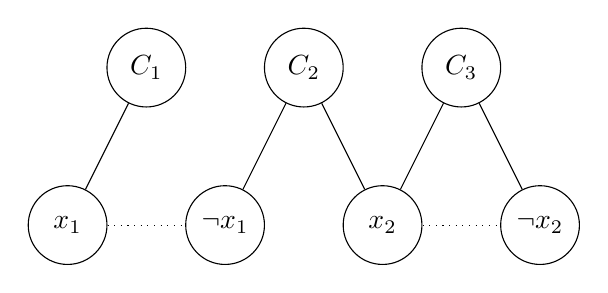
\begin{tikzpicture}[
        every node/.style={draw, circle, minimum size=1cm},
        node distance=1.5cm,
        scale=0.8,
    ]
        % Define Literal Nodes
        \node (x1) at (0, 0) {\(x_1\)};
        \node (notx1) at (2.5, 0) {\(\neg x_1\)};
        \node (x2) at (5, 0) {\(x_2\)};
        \node (notx2) at (7.5, 0) {\(\neg x_2\)};
        
        % Define Clause Nodes (one level above literals)
        \node[circle, draw] (C1) at (1.25, 2.5) {\(C_1\)};
        \node[circle, draw] (C2) at (3.75, 2.5) {\(C_2\)};
        \node[circle, draw] (C3) at (6.25, 2.5) {\(C_3\)};
        
        % Draw Edges (Literal → Clause)
        \draw (x1) -- (C1);
        \draw (notx1) -- (C2);
        \draw (x2) -- (C2);
        \draw (notx2) -- (C3);
        \draw (x2) -- (C3);
        
        % Draw Dotted Edges between each literal and its co mplement
        \draw[dotted] (x1) -- (notx1);
        \draw[dotted] (x2) -- (notx2);
    \end{tikzpicture}
    \caption{LCG representation of $\psi(V)$ with dashed lines representing the connection between complementary literals relevant for the message passing in GNNs.}
    \label{fig:lcg-sat}
\end{figure}

%\subsection{Incidence/Levi graph?}
%Defined in ALYAHYA et al. Concrete graphical representation of SAT? Type of bipartite graph.
%Defines edges via edge weight function! PART OF GRAPH THEORY \\
%Definition in Cimatti et al. : For clause $c$ we use $lit(c)$ and $var(c)$ to reference the %set of literals and variables in $c$ respectively. "$For a CNF formula F we write
%cla(F) for its set of clauses, lit(F)= c \in cla(F) lit(c) for its set of literals, and
%var(F)= c \in cla(F) var(c) for its set of variables.$"  Incidence graph of $\psi$ is the %bipartite graph $inc(\psi) = (V,E)$ with $V=lit(\psi) \cup cla(\psi)$. Additionally for %literal $x \in lit(\psi)$ and clause $c \in cla(\psi)$ we define $xc \in E$ if $x \in var(c)$.

\subsection{Unsatisfiable Cores}
The core of an unsatisfiable formula in CNF is a subset of the formula that is also unsatisfiable. Every unsatisfiable formula therefore is a core on its own, but can be broken down into smaller cores. The smaller a core the more significance it holds. A minimal unsatisfiable core is also referred to as a minimal unsatisfiable subset (MUS). SAT solvers like minisat\cite{} are able to compute unsatisfiable cores but do not generally provide a MUS due to high computational cost. However, several deletion-based algorithms exist for computing MUSs. Cuellar et al \cite{}

\subsection{Backbones}
Leave out for now.

\section{TODO NeuroSAT}
Machine learning approach for SAT solving using message passing neural network.
NeuroSAT: Messages are passed between clauses and literals, as well as literals and their complement. 1. Clause receives from neighboring literals 2. Literals receive from clauses and complement. \\
(Define flip function that swaps literal row with row of its negation; relevant for NeuroSAT)
    \chapter{Related Work}

%Propose only using PGExplainer for Node classification task.\bigskip
Yuan et al. \cite{yuan2022explainability} performed an extensive taxonomic survey on explainability in graph neural networks. We use this survey to discuss different approaches and motivate the selection of the PGExplainer in Section \ref{sec:gnn_explainability}. The authors note that the PGExplainer "is not performing as promising as its original reported results" \cite{yuan2022explainability}. Nevertheless, we evaluate the explainer model with regard to its applicability in the inductive setting. In Section \ref{sec:Explainer_Models} we briefly introduce important work related to the PGExplainer, as well as the model itself, since it is the core of our work. Lastly, we refer to NeuroSAT, which we use as a downstream model for the PGExplainer to generate explanations for its predictions on the SAT problem in Section \ref{sec:Downstream_Models}.

\section{Explainability in GNNs}
\label{sec:gnn_explainability}

Methods in DL have seen growth in performance in many tasks of artificial intelligence, including GNNs, since graphs are able to capture real-world data such as social networks or chemical molecules \cite{ying2018graph}, \cite{ma2021deep}. However, the interpretability of these models is often limited due to their black-box design \cite{noor2024survey}. Explainability methods aim to bypass this limitation by designing post-hoc techniques that provide insights into the decision-making process in the form of explanations. Such human-intelligible explanations are crucial for deploying models in real-world applications, especially when applied in interdisciplinary fields \cite{ribeiro2016should}.

There exist several different approaches for explaining predictions of deep graph models, that can be categorized into instance-level methods and model-level methods (see Yuan et al.  \cite{yuan2022explainability}). Instance-level methods aim to explain each input-graph by identifying important input features for its prediction, leading to input-dependent explanations. These can further be grouped by their importance score calculation into four branches. Gradients/feature-based methods use gradients as approximations of importance scores. Sensitivity Analysis \cite{baldassarre2019explainability} is an example that directly uses squared values of gradients as importance scores of input features. This enables the scores to be calculated directly with back-propagation.

Perturbation-based approaches like GNNExplainer \cite{ying2019gnnexplainer} and PGExplainer \cite{luo2020parameterized} study the variation of the output with regard to different input perturbations. The intuition behind this is that when input information crucial to the prediction is kept, the new prediction should roughly align with the prediction from the original input. PGExplainer aims to improve the GNNExplainer by providing a way of generating explanations with a global understanding of the GNN, significantly improving the computational cost. Another approach is SubgraphX \cite{yuan2021explainability}, which utilizes Monte Carlo Tree search to generate subgraph-level explanations. This does however entail a higher computational cost. 

Surrogate methods for deep graph models are inspired by surrogate methods for image data, that rely on neighboring areas of an input. Since graph data is concrete and contains topological information it is difficult to define the neighboring regions of an input graph. The idea is to obtain a local dataset containing neighboring data objects and predictions and fitting a simple, interpretable surrogate model to learn the local dataset. The explanations of the surrogate model are then regarded as the explanations of the original model. GraphLime \cite{huang2022graphlime} is an example that considers the $N$-hop neighboring nodes of a target node as the local dataset, where $N$ may be the number of GNN-layers. The weighted features of a non-linear surrogate model are then regarded as explanations. However, this method only explains node features, rather than the graph structure.

Decomposition methods, also motivated by success in the image domain, aim to measure input feature importance by decomposing the prediction into several terms, regarded as feature dependant importance score. Approaches for deep graph neural networks, like Layer-wise Relevance Propagation \cite{baldassarre2019explainability}, decompose the output prediction score to node importance scores. The decomposition rule is based on hidden features and weights, only enabling the study of node importance rather than graph structures.

Model-level methods, on the other hand, aim to explain GNNS without considering specific inputs, leading to input-independent, high-level explanations.


To fully trust the explanations provided by an explainer model, they must satisfy certain criteria, since there often is a mismatch between the optimizable metrics like accuracy and the actual metric of interest, which may not be measurable (see Ribeiro et al. \cite{ribeiro2016should}). First and foremost, an explanation should be \textbf{interpretable} and therefore provide qualitative, human-understandable interpretations, that also consider the possibility of limited user knowledge. Additionally, \textbf{local fidelity} asserts that explanations should be faithful in a local context and consider the models' behavior in the vicinity of predicted instances. Explainers that treat the model to be explained as a black-box are \textbf{model-agnostic} and should therefore be able to explain any model. Lastly, a \textbf{global perspective} is needed to explain a model fully, allowing us to take sample explanations of individual predictions that serve as representation of the model.

TODO: Claims to satisfy?
Since the perturbation-based PGExplainer \cite{luo2020parameterized} claims to satisfy all the criteria, while also maintaining reasonable computational cost, we select this model for the course of this study. It is furthermore able to generate explanations in an inductive setting, which we aim to do in \ref{}.

The general pipeline for different perturbation based approaches (see Figure \ref{fig:perturbation_pipeline}) can be described as follows: First, the important features from the input graph are converted into a mask by our generation algorithm, depending on the explanation task at hand. These masks are applied to the input graph to highlight said features. Lastly, the masked graph is fed into the trained GNN to evaluate the mask. The mask generation algorithm is updated according to the similarity of the predictions on the original and masked graphs. 

These different approaches mostly differ in the specific mask generation algorithm, the type of mask used and the objective function. It is important to distinguish between soft masks, discrete masks and approximated discrete masks. Soft masks take continuous values between $[0,1]$ which enables the graph algorithm to be updated via backpropagation. A downside of soft masks is that they suffer from the "introduced evidence" problem (see Dabkowski et al. \cite{dabkowski2017real}). Any mask value that is non-zero or non-one may add new semantic meaning or noise to the input graph, since graph edges are by nature discrete. Discrete masks however always rely on non-differentiable operations, e.g. sampling. Thus, the approximated discrete masks utilize reparameterization tricks to avoid the "introduced evidence" problem while also enabling back-propagation. %TODO: Expand on reparameterization trick?

Explanations can on the one hand be evaluated by visualizing the graph and considering the "human-comprehensibility". Since this requires a ground truth, is prone to the subjective understanding and is usually performed for a few random samples, it is important to apply stable evaluation metrics. One relevant accuracy metric for synthetic datasets with ground truths is the Area Under the Receiver Operating Characteristic Curve (ROC-AUC) (see Richardson et al. \cite{RICHARDSON2024100994}). The Receiver Operating Characteristic (ROC) curve plots the False Positive Rate (FPR) on the x-axis against the True Positive Rate (TPR), across different classification thresholds. The area under the curve (AUC) is calculated for said curve, resulting in the ROC-AUC, also referred to as AUROC. It is important to note, that a value of $0.5$ equals random guessing, while a score of $1.0$ indicates perfect classification. TODO: Other metrics include fidelity, results of taxonomy propose only using PGExplainer for Node Classification as it achieves low fidelity on Graph tasks

TODO: figure of perturbation pipeline?
\begin{figure}
    \includegraphics[width=\textwidth]{img/perturbation_pipeline.png}
    \caption{\small General pipeline of perturbation-based methods with a soft mask for node features, a discrete mask for edges, and an approximated discrete mask for nodes. The prediction of the GNN for the masked input graph is used in the objective function to train the generation algorithm and learn explanations. Reprinted from \cite{yuan2022explainability}.}
    \label{fig:perturbation_pipeline}
\end{figure}

\section{TODO: SECTION NAME Explainer Models}
\label{sec:Explainer_Models}

\textbf{GNNExplainer} \\
Ying et al. proposed the GNNExplainer \cite{ying2019gnnexplainer} - the first general, model-agnostic explainer for graph neural networks on any graph-based machine learning task. It is able to identify a concise subgraph structure and a subset of node features, that play a crucial role in the prediction of the underlying graph neural network. This is generally understood as an explanation. The work by Ying et al. serves as the main baseline for the PGExplainer, that seeks to improve its predecessor. Many concepts, experiments and specifications of PGExplainer were adapted from the GNNExplainer, which we seek to process in our work. \bigskip

\textbf{Parameterized Explainer for Graph Neural Networks} \\
The Parameterized Explainer for Graph Neural Networks (PGExplainer) by Lou et al. \cite{luo2020parameterized} is the main subject of our work. The idea of the framework is to collectively explain predictions of GNNs on a set of instance, while at the same time being able to generalize the explainer model to unexplained instances in an inductive setting. To achieve this, the method adapts a deep neural network to parameterize the generation process of explanations. %The method adopts a deep neural network to parameterize the generation process of explanations, thus allowing multiple instances to be explained collectively. Furthermore, it has better generalization ability and can explicitly be utilized in an inductive setting.

We reimplement the original work using PyTorch \cite{paszke2019pytorch} and PyTorch Geometric \cite{Fey/Lenssen/2019} instead of TensorFlow \cite{tensorflow2015-whitepaper}, while also emphasizing its application in an inductive setting, where test instances are unseen during training, as opposed to the original collective setting. A secondary study on the inductive performance was also performed by the authors, which we want to extend by applying it on a graph neural network with a slightly different architecture, testing whether the explainer proves to be model-agnostic. The goal of this thesis is to apply the explainer model to a deep learning approach for solving a bipartite graph problem - specifically, the boolean satisfiability problem - and generate proofs for the deep model's predictions. \bigskip

%This extension is motivated by the need for explainability methods that generalize across architectures (TODO: SOURCE FOR THIS).

\textbf{[Re] Parameterized Explainer for Graph Neural Network} \\
%We try own reimplementation that follows the original paper, as well as code and reimplementation for uncertainties + use a slightly different architecture in underlying GNN + Hyperparameter search of combination of parameters used in original and repication. Treated as additional baseline
Holdijk et al. \cite{holdijk2021re} performed a replication study on the PGExplainer that focuses on reimplementing the method in PyTorch, testing whether the claims with respect to the GNNExplainer hold and discussing whether the used evaluation method makes sense. They highlight a large discrepancy between the paper and codebase, making a replication that includes the evaluation method from the paper alone impossible. With help of the codebase, the authors are able to replicate the experiments and verify the main claims of the original paper. However, they express some concerns regarding the evaluation setup and note a large difference between the originally noted AUC scores and their results for most of the datasets. Additionally, they question the general approach for evaluating graph data with ground truths, as done in GNNExplainer and PGExplainer, which we will discuss in \ref{}. We use this work as an additional baseline for our approach, but note that the replication was also done in the collective setting. Therefore, the difference to our work lies mainly in the architecture used for the downstream model and the setting of the experiments.


\section{TODO: SECTION NAME Downstream Model}
\label{sec:Downstream_Models}

\textbf{NeuroSAT} \\
NeuroSAT by Selsam et al. \cite{selsam2018learning} is a machine learning approach for solving the boolean satisfiability problem using a message passing neural network. It is able to detect satisfying assignments, but lacks proofs of unsatisfiability. The authors performed a small study on the detection of unsat cores, revealing that NeuroUNSAT is able to detect UNSAT cores if the UNSAT problems contain a specific UNSAT core. However, this is expected to be due to the model memorizing the unsat cores, rather than generalizing to any unsat core. We want to test this by applying the PGExplainer in an inductive setting to the NeuroSAT model, and evaluate whether the generated explanations do align with unsat cores.
    \chapter{PGExplainer - Main part}
\label{ch:PGExplainer}
TODO: This can be understood as an extension of the theoretical background?

V1: In the following chapter, we introduce the PGExplainer\cite{luo2020parameterized} and its concepts. The idea is to generate explanations in the form of probabilistic graph generative models for any learned GNN model, henceforth referred to as the downstream task (DT), by utilizing a deep neural network to parameterize the generation process. This approach seeks to explain multiple instances collectively, as they share the same neural network parameters, and therefore improve the generalizability to previous works, particularly the GNNExplainer\cite{ying2019gnnexplainer}.

V2: In the following chapter, we introduce the PGExplainer\cite{luo2020parameterized} and its concepts. The idea is to generate explanations in the form of probabilistic graph generative models that have proven to learn the concise underlying structures of GNNs most relevant to their predictions. This approach may be applied to any learned GNN model, henceforth referred to as the downstream task (DT), by utilizing a deep neural network to parameterize the generation process. PGExplainer seeks to explain multiple instances collectively, as they share the same neural network parameters, and therefore improve the generalizability to previous works, particularly the GNNExplainer\cite{ying2019gnnexplainer}. This means that all edges in the dataset are predicted by the same model, which leads to a global understanding of the DT.

V3: In the following chapter, we introduce the PGExplainer\cite{luo2020parameterized} and its concepts. The idea is to generate explanations in the form of edge distributions or soft masks using a probabilistic generative model for graph data, known for being able to learn the concise underlying structures from the observed graph data. The explainer uncovers said underlying structures, believed to have the biggest impact on the prediction of a GNNs, as explanations. This approach may be applied to any trained GNN model, henceforth referred to as the target model (TM). 
By utilizing a deep neural network to parameterize the generation process, the explainer learns to collectively explain multiple instances of a model. Since the parameters of the neural network are shared across the population of explained instance, PGExplainer provides "model-level explanations for each instance with a global view of the GNN model". Furthermore, this approach cannot only be used in a transductive setting, but also in an inductive setting, where explanations for unexplained nodes can be generated without retraining the explanation model. This improves the generalizability compared to previous works, particularly the GNNExplainer\cite{ying2019gnnexplainer}.

The focus in this approach lies in explaining the graph structure, rather than the graph features, as feature explanations are already common in non-graph neural networks. \\

Transductive/Inductive explanation? \\

We then describe our reimplementation in detail (Section 3.2), including the changes made and difficulties during the process. \\

In Section 3.3 we present the idea of applying PGExplainer on the NeuroSAT framework to generate explanations for the machine learning SAT-solving approach and comparing these to "human-understandable" concepts like UNSAT cores and backbone variables. 
%Usable in transductive and inductive settings, the latter being the reason for better generalizability, as the explainer model does not have to be retrained to infer explanations of unexplained nodes.
\section{Theory}
We follow the structure of the original paper\cite{} and start by describing the learning objective (Section 3.1.1), the reparameterization trick (Section 3.1.2), the global explanations (Section 3.1.3) and regularization terms (Section 3.1.4).

\subsection{Learning Objective}
To explain the predictions made by a GNN model for an original input graph $G_o$ with $m$ edges we first define the graph as a combination of two subgraphs: $G_o = G_s + \Delta G$, where $G_s$ represents the subgraph holding the most relevant information for the prediction of a GNN, referred to as explanatory graph. $\Delta G$ contains the remaining edges that are deemed irrelevant for the prediction of the GNN. Inspired by GNNexplainer\cite{ying2019gnnexplainer}, the PGExplainer then finds $G_s$ by maximizing the mutual information between the predictions of the target model and the underlying $G_s$:
\begin{equation}
    \max_{G_s} I(Y_o;G_s) = H(Y_o) - H(Y_o|G=G_s),
\end{equation} 
where $Y_o$ is the prediction of the target model with $G_o$ as input. This quantifies the probability of prediction $Y_o$ when the input graph is restricted to the explanatory graph $G_s$, as in the case of $I(Y_o;G_s) = 1$, knowing the explanatory graph $G_s$ gives us complete information about $Y_o$, and vice versa. Intuitively, if removing an edge $(i,j)$ changes the prediction of a GNN drastically, this edge is considered important and should therefore be included in $G_s$. This idea originates from traditional forward propagation based methods for whitebox explanations (see Dabkowski et al.\cite{dabkowski2017real}).
It is important to note that $H(Y_o)$ is only related to the target model with fixed parameters during the evaluation/explanation stage. This leads to the objective being equivalent to minimizing the conditional entropy $H(Y_o|G=G_s)$.

To optimize this function a relaxation is applied for the edges, since normally there would be $2^m$ candidates for $G_s$. The explanatory graph is henceforth assumed to be a Gilbert random graph, where the selections of edges from $G_o$ are conditionally independent to each other. However, the authors describe a random graph with each edge having its own probability, rather than a shared probability as described in \ref{sec:random-graphs}, as follows: Let $e_{ij}\in V \times V$ be the binary variable indicating whether the edge is selected, with $e_{ij} = 1$ if edge $(i,j)$ is selected to be in the graph, and 0 otherwise. For the random graph variable $G$ the probability of a graph $G$ can be factorized as 
\begin{equation}
    P(G) = \prod_{(i,j)\in E}P(e_{ij}).
\end{equation}
TODO: Inhomogeneous Erdos Renyi model? Mention that this is a generative model?
 $P(e_{ij})$ is instantiated with the Bernoulli distribution $e_{ij} \sim Bern(\theta_{ij})$, where $P(e_{ij} = 1) = \theta_{ij}$ is the probability that edge $(i,j)$ exists in $G$.
After this relaxation the learning objective becomes:
\begin{equation}
    \label{eq:init_learning_obj}
    \min_{G_s}H(Y_o|G = G_s) = \min_{G_s} \mathbb{E}_{G_s}[H(Y_o|G = G_s)] \approx \min_{\Theta} \mathbb{E}_{G_s \sim q(\Theta)}[H(Y_o|G = G_s)],
\end{equation}
where $q(\Theta)$ is the distribution of the explanatory graph that is parameterized by $\Theta$'s.

\subsection{Reparameterization Trick}
As described in section \ref{sec:perturbation-based_explainability}, a reparameterization trick can be utilized to relax discrete edge weights to continuous variables in the range $(0,1)$. PGExplainer uses the reparameterizable Gumbel-Softmax estimator\cite{jang2016categorical} to allow for efficiently optimizing the objective function with gradient-based methods. This method introduces the Gumbel-Softmax distribution, a continuous distribution used to approximate samples from a categorical distribution. A temperature $\tau$ is used to control the approximation, usually starting from a high value and annealing to a small, non-zero value. Samples with $\tau > 0$ are not identical to samples from the corresponding continuous distribution, but are differentiable and therefore allow back-propagation. The sampling process $G_s \sim q(\Theta)$ of PGExplainer is therefore approximated with a determinant function that takes as input the parameters $\Omega$, a temperature $\tau$ and an independent random variable $\epsilon$: $G_s \approx \hat{G}=f_\Omega(G_o,\tau,\epsilon)$. The binary concrete distribution\cite{maddison2016concrete}, also referred to as Gumbel-Softmax distribution, is utilized as an instantiation for the sampling, yielding the weight $\hat{e}_{ij} \in (0,1)$ for edge $(i,j)$ in $\hat{G}_s$, computed by:
\begin{equation}
    \label{eq:reparam_trick}
    \epsilon \sim \text{Uniform}(0,1), \qquad \hat{e}_{ij}=\sigma((\log \epsilon - \log(1-\epsilon)+\omega_{ij}/\tau),
\end{equation}
where $\sigma(\cdot)$ is the Sigmoid function and $\omega_{ij} \in \mathbb{R}$ is an explainer logit for the corresponding edge used as a parameter. When $\tau \rightarrow 0$, e.g. during the explanation stage, the weight $\hat{e}_{ij}$ is binarized with the sigmoid function $\lim_{\tau\rightarrow 0}P(\hat{e}_{ij} = 1) = \frac{\exp (\omega{ij})}{1+\exp (\omega{ij})}$. Since $P(e_{ij} = 1) = \theta_{ij}$, choosing $\omega_{ij} = \log\frac{\theta_{ij}}{1-\theta_{ij}}$ leads to $\lim_{\tau\rightarrow 0}\hat{G}_s = G_s$ and justifies the approximation of the Bernoulli distribution with the binary concrete distribution. During training, when $\tau > 0$, the objective function in \eqref{eq:init_learning_obj} is smoothed with a well-defined gradient $\frac{\partial\hat{e}_{ij}}{\partial\omega_{ij}}$ and becomes:
\begin{equation}
    \min_\Omega \mathbb{E}_{\epsilon \sim \text{Uniform}(0,1)}H(Y_o| G = \hat{G}_s)
\end{equation}

The authors follow the approach of GNNExplainer\cite{ying2019gnnexplainer} and modify the objective by replacing the conditional entropy with cross entropy between the label class and the prediction of the target model. This is justified by the greater importance of understanding the model's prediction of a certain class, rather than providing an explanation based solely on its confidence.

With the modification to cross-entropy $H(Y_o, \hat{Y}_s)$, where $\hat{Y}_s$ is the prediction of the target model when $\hat{G}_s$ is given as input, as well as the adaption of Monte Carlo sampling, the learning objective becomes:
TODO: ONE LABEL FOR BOTH EQUATIONS!?
\begin{align}
    \label{eq:monte_carlo}
    &\min_\Omega\mathbb{E}_{\epsilon\sim\text{Uniform}(0,1)}H(Y_o, \hat{Y}_s) \approx \min_\Omega -\frac{1}{K}\sum_{k=1}^K\sum_{c=1}^C P(Y_o = c) \log P(\hat{Y}_s = c) \\
    = &\min_\Omega -\frac{1}{K}\sum_{k=1}^K\sum_{c=1}^C P_\Phi (Y_o = c|G = G_o) \log P_\Phi(\hat{Y}_s = c|G=\hat{G}_s^{(k)}).
\end{align}
$\Phi$ denotes the parameters in the target model, $K$ is the number of total sampled graphs, $C$ is the number of class labels, and $\hat{G}_s^{(k)}$ denotes the $k$-th graph sampled with equation \ref{eq:reparam_trick}, parameterized by $\Omega$. %Note that this objective is defined per explainable instance.



%The approach in PGExplainer is a common approach in ML for simplifying objectives? FIND LITERATURE THAT EXPLAINS APPROXIMATION OF COND. ENTROPY WITH CROSS ENTROPY. Explanation as simple as one formula for one graph variable example, cross entropy applied to whole distribution? \bigskip


\subsection{Global Explanations}
The novelty of PGExplainer lies in the ability to generate explanations for graph data with a global perspective, that allow for understanding the general picture of a model across a population. This saves resources when analyzing large graph datasets, as new instances can be explained without retraining the model, and can also be helpful for establishing the users' trust in these explanations. To achieve this the authors propose the use of a parameterized network that learns to generate explanations from the target model, which also apply to not yet explained instances. PGExplainer hence explains predictions of the target model over multiple instances collectively (TODO: Cut this sentence?).

Since GNNs apply two functions $F$ and $G$ to calculate the global state embeddings and downstream task outputs respectively, we denote these two functions as $\text{GNNE}_{\Phi_0}(\cdot)$ and $\text{GNNC}_{\Phi_1}(\cdot)$ for any GNN in the context of PGExplainer. For models without explicit classification layers the last layer is used to compute the output instead. It follows
\begin{equation}
    \mathbf{Z} = \text{GNNE}_{\Phi_0}(G_o, \mathbf{X}), \qquad Y = \text{GNNC}_{\Phi_1}(\mathbf{Z}),
\end{equation}
where $\mathbf{Z}$ denotes the matrix of final node representations $z$, referred to as node embeddings, and the initial state is $G_o$. TODO: (Because of focus on graph structure rather than features?) For generalizability across different GNN layers the output is only dependent on the node representation, that encapsulates both features and structure of the input graph. This representation also serves as the input for the explainer network $g$, defined as:
TODO: Rename g?
\begin{equation}
    \label{eq:explainer_network}
    \Omega = g_\Psi(G_o,\mathbf{Z}).
\end{equation}
$\Psi$ denotes the parameters in the explanation network and the output $\Omega$ is treated as parameter in equation \ref{eq:monte_carlo}. Since $\Psi$ is shared by all edges among the population, PGExplainer collectively provides explanations for multiple instances. Thus, the learning objective in a collective setting with $\mathcal{I}$ being the set of instances becomes:
\begin{equation}
    \min_\Psi -\frac{1}{K}\sum_{i\in \mathcal{I}}\sum_{k=1}^K\sum_{c=1}^C P_\Phi (Y_o = c|G = G_o^{(i)}) \log P_\Phi(\hat{Y}_s = c|G=\hat{G}_s^{(i,k)}).
\end{equation}
Consequently, $G^{(i)}$ and $G_s^{(i,k)}$ denote the input graph and the $k$-th graph sampled with equation \ref{eq:reparam_trick} in \ref{eq:explainer_network} respectively for instance $i$. The authors propose two slightly different instantiations for node classification and graph classification tasks. \bigskip

\textbf{Explanation network for node classification}
%Since explanations for different nodes may not share a common explanation pattern, especially for nodes with different labels, ... DOES THIS NOT ALSO APPLY FOR GRAPHS?!
TODO: Motivate the difference between these two tasks? Not done by authors \bigskip

Let an edge $(i,j)$ be considered relevant for the prediction of a node $u$, but irrelevant for the prediction of a node $v$. To explain the prediction of node $v$ we specify the network in \ref{eq:explainer_network} as:
\begin{equation}
    \omega_{ij} = \text{MLP}_\Psi ([\mathbf{z}_i\oplus\mathbf{z}_j\oplus\mathbf{z}_v]).
\end{equation}
$\text{MLP}_\Psi$ is an MLP (TODO see \ref{} for implementation details) parameterized with $\Psi$ and $\oplus$ denotes the concatenation operation. Thus, a concatenation of the node embeddings of nodes $i, j$ and $v$ respectively is fed through the network. The output $\omega_{ij}$ is therefore an edge logit, which serves as a parameter in the sampling process.

Note that in their codebase the authors use a concatenation of all hidden representations instead of final node embeddings for node level tasks.
For a target GNN consisting of multiple graph layers with
\begin{align*}
    \mathbf{H}_1 &= F_1(G_o, \mathbf{X}), \\
    \mathbf{H}_2 &= F_2(\mathbf{H}_1, \mathbf{X}), \\
    &\vdots \\
    \mathbf{H}_L &= F_L(\mathbf{H}_{L-1}, \mathbf{X}), \\
\end{align*}
this leads to $Z$ being the matrix of node embeddings $z$ that are computed as:
\begin{equation}
    z_i = h_{1,i} \oplus h_{2,i} \oplus ... \oplus h_{L,i}
\end{equation}

\textbf{Explanation network for graph classification}
For graph level tasks the authors consider each graph to be an instance, regardless of specific nodes. The specification for the network thus becomes:
\begin{equation}
    \omega_{ij} = \text{MLP}_\Psi ([\mathbf{z}_i\oplus\mathbf{z}_j]),
\end{equation}
where for each edge in $G_o$ a concatenation of both its nodes is fed through the MLP.\bigskip

TODO: Include computational complexity of PGE in comparison to GNN?

This leads to an improved computational complexity when compared to their baseline GNNExplainer, since for one the number of parameters in the explainer does no longer depend on the size of the input graph and since the explainer does not have to be retrained for every unexplained instance.

TODO: Include algorithms?

\tikzstyle{process} = [rectangle, rounded corners, minimum width=3cm, minimum height=1cm, text centered, draw=black, fill=purple!30, font=\small]
\tikzstyle{module} = [rectangle, rounded corners, minimum width=3cm, minimum height=1.2cm, text centered, draw=black, fill=gray!30, font=\small]
\tikzstyle{data} = [rectangle, sharp corners, minimum width=1.5cm, minimum height=1cm, text centered, draw=black, fill=cyan!30, font=\small]
\tikzstyle{emb} = [rectangle, sharp corners, minimum width=1.5cm, minimum height=1cm, text centered, draw=black, fill=yellow!30, font=\small]
\tikzstyle{arrow} = [very thick,->,>=Stealth]    %very thick

\begin{figure}
\centering
\begin{tikzpicture}[node distance=0.9cm and 1.2cm]

\tikzset{
  mymini/.pic={
    \node[circle, draw, fill=black, inner sep=2pt] (x) at (0,0) {};
    \node[circle, draw, fill=black, inner sep=2pt] (y) at (0.5,0.5) {};
    \node[circle, draw, fill=black, inner sep=2pt] (a) at (0,0.5) {};
    \node[circle, draw, fill=black, inner sep=2pt] (b) at (0,-0.5 ) {};
    \draw[-] (x) -- (y);
    \draw[-] (a) -- (y);
    \draw[-] (b) -- (x);
    \draw[-] (a) -- (x);
  }
}

\tikzset{
  mymini3/.pic={
    \node[circle, draw, fill=black, minimum size=4pt, inner sep=2pt, label=left:$z_i$] (x) at (0,0) {};
    \node[circle, draw, fill=black, minimum size=4pt, inner sep=2pt, label=above:$z_j$] (y) at (0.5,0.5) {};
    \node[circle, draw, fill=black, minimum size=4pt, inner sep=2pt, label=left:$z_k$] (a) at (0,0.5) {};
    \node[circle, draw, fill=black, minimum size=4pt, inner sep=2pt, label=left:$z_l$] (b) at (0,-0.5) {};
    \draw[-] (x) -- (y);
    \draw[-] (a) -- (y);
    \draw[-] (b) -- (x);
    \draw[-] (a) -- (x);
  }
}

\tikzset{
  mymini2/.pic={
    \node[circle, draw, fill=black, inner sep=2pt] (x) at (0,0) {};
    \node[circle, draw, fill=black, inner sep=2pt] (y) at (0.5,0.5) {};
    \node[circle, draw, fill=black, inner sep=2pt] (a) at (0,0.5) {};
    \node[circle, draw, fill=black, inner sep=2pt] (b) at (0,-0.5 ) {};
    \draw[-] (x) -- node[midway, right, font=\scriptsize] {$0.9$} (y);
    \draw[-] (a) -- node[midway, above, font=\scriptsize] {$0.8$}(y);
    \draw[-] (b) -- node[midway, left, font=\scriptsize] {$0.1$}(x);
    \draw[-] (a) -- node[midway, left, font=\scriptsize] {$0.9$}(x);
  }
}

\tikzset{
  mymini4/.pic={
    \node[circle, draw, fill=black, inner sep=2pt] (x) at (0,0) {};
    \node[circle, draw, fill=black, inner sep=2pt] (y) at (0.5,0.5) {};
    \node[circle, draw, fill=black, inner sep=2pt] (a) at (0,0.5) {};
    \node[circle, draw, fill=black, inner sep=2pt] (b) at (0,-0.5 ) {};
    \draw[-] (x) -- node[midway, right, font=\scriptsize] {$z_{ij}$} (y);
    \draw[-] (a) -- node[midway, above, font=\scriptsize] {$z_{jk}$}(y);
    \draw[-] (b) -- node[midway, left, font=\scriptsize] {$z_{il}$}(x);
    \draw[-] (a) -- node[midway, left, font=\scriptsize] {$z_{ik}$}(x);
  }
}

\tikzset{
  mymini5/.pic={
    \node[circle, draw, fill=black, inner sep=2pt] (x) at (0,0) {};
    \node[circle, draw, fill=black, inner sep=2pt] (y) at (0.5,0.5) {};
    \node[circle, draw, fill=black, inner sep=2pt] (a) at (0,0.5) {};
    \node[circle, draw, fill=black, inner sep=2pt] (b) at (0,-0.5 ) {};
    \draw[-] (x) -- (y);
    \draw[-] (a) -- (y);
    \draw[-] (a) -- (x);
  }
}


% Nodes
\node (input) [data] {\small Input Graph $G_o$};
\pic at ([xshift=7cm]input.center) {mymini};
\node (target) [module, below=of input] {Target GNN};
\node (embeddings) [emb, below=of target] {Node Embeddings $\mathbf{Z}$ of $G_o$};
\node[anchor=center] at ([xshift=4cm]embeddings.center) 
 (node_embs) 
 {$\begin{bmatrix} z_i \\ z_j \\ \vdots \end{bmatrix}$};
\node[right=0.01cm of node_embs, anchor=west] 
 {\scriptsize $[|V(G_o)|]$};
\pic at ([xshift=7cm]embeddings.center) {mymini3};
\node (embedding_transformation) [process, below=of embeddings] {Edge Embedding Transformation};
\node (edge_embeddings) [emb, below=of embedding_transformation] {Edge Embeddings of $G_o$};
\node[anchor=center] at ([xshift=4cm]edge_embeddings.center) 
 (edge_embs) 
 {$\begin{bmatrix} z_{ij} \\ z_{jk} \\ \vdots \end{bmatrix}$};
\node[right=0.01cm of edge_embs, anchor=west] 
 {\scriptsize $[|E(G_o)|]$};
\pic at ([xshift=7cm]edge_embeddings.center) {mymini4};
\node (explainer) [module, below=of edge_embeddings] {PGExplainer MLP};
\node (logits) [emb, below=of explainer] {Edge Logits/Latent variables $\Omega$};
\node[anchor=center] at ([xshift=4cm]logits.center) 
 (omega) 
 {$\begin{bmatrix} \omega_{ij} \\ \omega_{jk} \\ \vdots \end{bmatrix}$};
\node[right=0.01cm of omega, anchor=west] 
 {\scriptsize $[|E(G_o)|]$};
\node (trick) [process, below=of logits] {Reparameterization Trick};
\node (weights) [emb, below=of trick] {Sampled edge importance weights};
\node[anchor=center] at ([xshift=4cm]weights.center) 
 (edge_score) 
 {$\begin{bmatrix} \hat{e}_{ij} \\ \hat{e}_{jk} \\ \vdots \end{bmatrix}$};
\node[right=0.01cm of edge_score, anchor=west] 
 {\scriptsize $[|E(G_o)|]$};

\node (sampled_graph) [data, below= of weights] {Sampled graph $\hat{G}_s$};
\pic at ([xshift=7cm]sampled_graph.center) {mymini2};

\node (sample_target) [module, below=of sampled_graph] {Target GNN};
\node (original_target) [module, left=2cm of sample_target] {Target GNN};
\node (sample_prediction) [data, below=of sample_target] {$\hat{Y}_s$};
\pic at ([xshift=7cm]sample_prediction.center) {mymini5};
\node (original_prediction) [data, below=of original_target] {$Y_o$};

\node (topK) [process, right=of sample_target] {Sample top-$k$ edges};
\node (explanation) [data, below=of topK] {$G_s$};

%\node[draw=red, thick, dashed, fit=(input) (target) (embeddings), label=above:input Block] {};

%\begin{pgfonlayer}{background}
%    \node[draw=gray, thick, rounded corners, fit=(edge_embeddings) (weights), fill=blue!10, label=above:Sampling of PGExplainer] {};
%\end{pgfonlayer}

\begin{pgfonlayer}{background}
    \node[draw=gray, thick, rounded corners, fit=(original_target) (sample_target) (original_prediction) (sample_prediction), fill=orange!30, label=above:Training] {};
\end{pgfonlayer}

\begin{pgfonlayer}{background}
    \node[draw=gray, thick, rounded corners, fit=(topK) (explanation), fill=green!30, label=above:Evaluation] {};
\end{pgfonlayer}

\coordinate (weight_sample_mid) at ($ (weights)!0.5!(sampled_graph) $);
\coordinate (left_of_input) at ($ (input) + (-3.5cm, 0) $);
\coordinate (right_of_input) at ($ (original_target |- input) $);
\coordinate (drop) at (left_of_input |- weight_sample_mid);
\coordinate (right_of_sampled_graph) at ($ (topK |- sampled_graph) $);

% Arrows
\draw [arrow] (input) -- (target);
\draw [arrow] (target) -- (embeddings);
\draw [arrow] (embeddings) -- (embedding_transformation);
\draw [arrow] (embedding_transformation) -- (edge_embeddings);
\draw [arrow] (edge_embeddings) -- (explainer);
\draw [arrow] (explainer) -- (logits);
\draw [arrow] (logits) -- (trick);
\draw [arrow] (trick) -- (weights);

%\draw [arrow] (input.west) --  ++(-2cm,0) -- ($ (input) + (-2cm,0) $ |- sampled_graph) -- (sampled graph.west);
\draw [arrow] (weights) -- (sampled_graph);

\draw[arrow] 
  (input) -- (left_of_input) 
       -- (drop) 
       -- (weight_sample_mid);

\draw[arrow] 
  (left_of_input) -- (right_of_input) 
       -- (original_target);

\draw [arrow] (sampled_graph) -- (sample_target);
\draw [arrow] (sample_target) -- (sample_prediction);

\draw [arrow] (original_target) -- (original_prediction);

\draw [arrow] (sampled_graph) -- (right_of_sampled_graph) -- (topK);

\draw [arrow] (topK) -- (explanation);

\draw [<->, dashed] (sample_prediction) -- node[midway, above, font=\scriptsize] {$\min_\Omega H(Y_o,\hat{Y}_s)$} (original_prediction);

\end{tikzpicture}
\caption{Test}
\end{figure}

\begin{figure}
\centering
\begin{tikzpicture}
    
    \node (node_emb_i1) [data] {$z_i$};
    \node (node_emb_j1) [data, right=0.5cm of node_emb_i1] {$z_j$};
    
    \coordinate (i_j_mid) at ($ (node_emb_i1)!0.5!(node_emb_j1) $);
    
    \node (concat) at ($(i_j_mid) + (0,-1)$) {\Large $\oplus$};
    
    \node (edge_emb_ij) [data] at ($(i_j_mid) + (0,-2)$) {Edge Embedding of $(i,j)$};
    
    
    \node (node_emb_i2) [data, right=3cm of node_emb_j1] {$z_i$};
    \node (node_emb_j2) [data, right=0.5cm of node_emb_i2] {$z_j$};
    \node (node_emb_v2) [data, right=0.5cm of node_emb_j2] {$z_v$};
    
    \coordinate (i_v_mid) at ($ (node_emb_i2)!0.5!(node_emb_v2) $);
    
    \node (concat2) at ($(i_v_mid) + (0,-1)$) {\Large $\oplus$};
    
    \node (edge_emb_ijv) [data] at ($(i_v_mid) + (0,-2)$) {Edge Embedding of $(i,j)$ with target node $v$};


    \node (z_i) [data, above=2cm of node_emb_j2] {$z_i$};

    \node (h_2) [data, above=1cm of z_i] {$h_{2,i}$};
    \node (h_1) [data, left=0.5cm of h_2] {$h_{1,i}$};
    \node (h_3) [data, right=0.5cm of h_2] {$h_{3,i}$};
 
    \node (O) [module, above=1cm of h_2] {$O$};
    \node (F_3) [module, above=0.2cm of O] {$F_3$};
    \node (F_2) [module, above=0.2cm of F_3] {$F_2$};
    \node (F_1) [module, above=0.2cm of F_2] {$F_1$};
    \node (H_2) [data, right=0.5cm of F_2] {$H_2 = [h_{2,i}, h_{2,j},...]$};
    \node (H_1) [data, right=0.5cm of F_1] {$H_1 = [h_{1,i}, h_{1,j},...]$};
    \node (H_3) [data, right=0.5cm of F_3] {$H_3 = [h_{3,i}, h_{3,j},...]$};

    \node (input) [data, above=1cm of F_1] {$G_o$};

    \node (concat3) at ($ (h_2 |- z_i) + (0,1)$) {\Large $\oplus$};

    \begin{pgfonlayer}{background}
        \node[draw=gray, thick, rounded corners, fit=(F_1) (O) (H_1), fill=gray!30, inner sep=20pt, label=above:\text{Target GNN}] {};
    \end{pgfonlayer}



    \begin{pgfonlayer}{background}
        \node[draw=purple, dashed, rounded corners, fit=(node_emb_i1) (node_emb_j1) (node_emb_i2)(node_emb_v2) (edge_emb_ijv), inner sep=20pt, label=above:\text{Edge Embedding Transformation}] {};
    \end{pgfonlayer}
    
    \begin{pgfonlayer}{background}
        \node[draw=gray, thick, rounded corners, fit=(node_emb_i1) (node_emb_j1) (edge_emb_ij), fill=red!30, label=above:Graph Task] {};
    \end{pgfonlayer}
    
    \begin{pgfonlayer}{background}
        \node[draw=gray, thick, rounded corners, fit=(node_emb_i2) (node_emb_v2) (edge_emb_ijv), fill=orange!30, label=above:Node Task] {};
    \end{pgfonlayer}
\end{tikzpicture}
\caption{Visualization of the edge embedding transformation used to create inputs for the explainer network. Depending on the downstream task used in the target model the created edge embedding differs slightly.}
\end{figure}

\subsection{Regularization Terms}
To enhance the preservation of desired properties of explanations the authors propose various regularization terms. These are added to the learning objective, depending on the specific downstream task at hand.\bigskip

\textbf{Size and entropy constraints}

Inspired by GNNExplainer\cite{ying2019gnnexplainer}, to obtain compact and precise explanations, a constraint on the size of the explanations is added in the form of $||\Omega||_1$, the $l_1$ norm on latent variables $\Omega$. Additionally, to encourage the discreteness of edge weights, element-wise entropy is added as a constraint:
\begin{equation}
    H_{\hat{G}_s} = -\frac{1}{|\varepsilon|}\sum_{(i,j)\in \varepsilon} (\hat{e}_{ij}\log \hat{e}_{ij} + (1-\hat{e}_{ij})\log(1-\hat{e}_{ij})),
\end{equation}
for one explanatory graph $\hat{G_s}$ with $\varepsilon$ edges. For the collective setting, this is added as a mean over all instances in $\mathcal{I}$. \bigskip

Note that the following two constraints are not used in the original experimental setup, but serve as inspiration for constraints introduced in our NeuroSAT application\ref{} and are therefore included. \bigskip

\textbf{Budget constraint}

The authors propose the modification of the size constraint to a budget constraint, for a predefined available budget $B$. Let $|\hat{G}_s| \leq B$, then the budget regularization is defined as:
\begin{equation}
    R_b = \text{ReLU}(\sum_{(i,j)\in \varepsilon}\hat{e}_{ij}-B).
\end{equation}
Note that $R_b = 0$ when the explanatory graph is smaller than the budget. When out of budget, the regularization is similar to that of the size constraint. \bigskip

\textbf{Connectivity constraint}

To enhance the effect of the explainer detecting a small, connected subgrap, motivated through real-life motifs being inherently connected, the authors suggest adding the cross-entropy of adjacent edges. Let $(i,j)$ and $(i,k)$ be two edges that both connect to the node $i$, then $(i,k)$ should rather be included in the explanatory graph if the edge $(i,j)$ is selected to be included. This is formally defined as:
\begin{equation}
    H(\hat{e}_{ij},\hat{e}_{ik}) = -[1-\hat{e}_{ij}\log(1-\hat{e}_{ik})+\hat{e}_{ij}\log \hat{e}_{ik}].
\end{equation}
We note that in practice this is implemented only for the two highest edge weights for each edge. The definition therefore would change to $(i,j)$ and $(i,k)$ being the top two edges that connect to node $i$.


\section{Reimplementation}
Notes on Original code of target model: Not clearly specified in paper, but according to code:
- No specific args set for layers etc., except hyperparameters for different datasets (see sweeps)
- Therefore, assuming default settings for layers -> Graph conv layer uses ReLu activation (done), bias initialized with zeroes (done), no dropout(partially done), and embedding normalization! (TODO), default order 'AW', weight init 'glorot' (Done with Xavier)
- WE USED PyG GraphConv since it allows for bipartite+edge weights; but compare to layer close to original!!\bigskip

Concrete graph layer used in original code is very similar to the semi-supervised layer\ref{}:
\begin{equation}
    Z = \hat{A}XW
\end{equation}
Note that a pytorch implementation of the semi-supervised layer is used in the replication paper:
\begin{equation}
    X' = \hat{D}^{-\frac{1}{2}}\hat{A}\hat{D}^{-\frac{1}{2}}X\Theta
\end{equation}
We use a pytoch implementation of the Weisfeiler and Leman Go Neural layer:
\begin{equation}
    x_i' = W_1x_i+W_2 \sum_{j\in\mathcal{N}(i)}e_{j,i}\cdot x_j
\end{equation}

TODO: Maybe separate the theory of PGE from our own work more strictly? E.g. 3. PGE theory, 4. PGE reimplementation and NeuroSAT application? \\
Implementation details:
\begin{itemize}
    \item Started by reimplementing the downstream tasks used in og paper for node and graph class.
    \item Node datasets taken from original and transformed to a "pyg format", to keep original structure and ground truths
    \item Graph: BA-2Motif from pyg library with self generated gt, MUTAG dataset taken from pyg and added gt-labels that were added in original dataset
    \item Created pytorch/pytorch geometric implementation of 3-layer graph conv networks
    \item architecture as described in paper: ReLu activation, Pooling for graph net
    \item Xavier initialization for all layers
    \item Same hyperparameters?(Adam, $1*10^-3$ lr, 1000 epochs)/experimental setup?
    \item ADDED Dropout(0.1) to improve performance/overfitting on node tasks
    \item Fully connected layer: torch geometric GraphConv to allow passing of edge weights(+ bipartite)!?
    \item Original references sageConv in paper, pyG impl. does not allow edge weights, verify!
    \item GATConv for Graph attention(referenced by original)
    \item Alternatives: GCNConv(edge weights, no bipartite graphs)
    \item 80/10/10 split
    \item => Similar accuracies achieved
\end{itemize}
 

 Explainer:
 This is irrelevant for paper, description of why reparameterization trick necessary
 - First approach tried passing a masked edge index to downstream task with edge weights > 0.5
 => Unable to learn with hard cut-off (bad for gradients). (Same with TopK probably?!)
 - Pass calculated edge weights to downstream task for learning. If no edge weights are passed(downstream task), all edge weights are initialized with one to represent all edges beeing relevant
 
%\section{Benchmarking}
%\section{Application on Bipartite Graphs?}#

\section{Application on NeuroSAT}
Reimplementation of NeuroSAT provided by Rodhi. As the code used for NeuroSAT can also be found in our Repository, we stress that only the changes described in the following chapter are part of our work. \\

What did we do? What did we change for NeuroSAT? What data was used? How did we adapt PGExplainer? \\

Only change in NeuroSAT: pass edge weights into adjacency matrix. Calculates .... \\
Generated batches of unsat problems that "turned" unsat because of last added clause. 10 literals per problem. Only unsat to test for unsat cores, that only apply for unsat problems. Calculated unsat cores with solver xy by adding negative assumption literals per clause and passing these as assumption for calulation. The edges of the clauses present in the unsat core were treated as ground truth. \\

Changes for explainer:
Edge embeddings calced by DS and passed to explainer. Calculated edge embeddings by concatenating node embeddings for connected nodes, similar to original. Embeddings fed into MLP, weights sampled with reparam. trick to get edge "probabilities", passed as "unbatched" sampled graph into NeuroSAT predictor. Visualization of SAT problems with edge weights, ands gts. \\
For quant. eval. adapted roc auc as metric as done in PGExplainer. Results seem "good" but qual. eval. shows different result. roc auc bad metric? \\
For qual. eval. topk(=number of edges in gt) edges of predictions were highlighted to be compared to gt edges. For quant. eval. the edge probabilites were compared to gt with 1s for edges in gt and 0s for rest. \\
    \include{chapters/05-implementation-details}
    \chapter{Results}
\label{ch:Results}

Experimental Setup:
We follow the experimental setup from the PGExplainer as closely as possible. Since the textual description refers to the setup from GNNExplainer and is lacking in some aspects, we extract the missing information from the codebase. As the hyperparameters are unclear or not comprehensible for some tasks we also draw information from the configs of PYTORCH REIMPL. \\

We use normalization in our downstream models, though it is not described in the paper, since it is used in the code. We also experimented with the effects of the use of normalization since it seems to be relevant to the performance of the explainer. \\
The explainer is trained and evaluated on the same data. We also run experiments with added train/test splits TODO! \\
Not all data is fed into the explainer:
BA-Shapes: 
BA-Community:
Tree-Cycles: "First"/to base graph attached node of each motif in graph is used.
Tree-Grid: All Motif nodes are used
BA-2Motif: All graphs are used
MUTAG: Only the graphs with an available ground truth are used. GT exist for mutagenic graphs that have either chemical groups NH2 or NO2.
We later discuss if these selections make sense and run experiments with different data selections.

Quantitative: 10 explainer runs on one downstream model; Calculate ROC-AUC over ALL graphs/nodes in each run;
Qualitative: Original uses a threshold; we instead take the topK nodes according to the dataset/motif as an explanation

We also discuss if treating the number of k edges as a hyperparameter dependant on the downstream task makes sense and propose having the network learn it, to improve generalizability and allow the explainer to work on data with varying size. \\

CPU vs GPU: \\
It is important to highlight that our code achieved better and way more stable results for BA-2Motif when trained on a gpu instead of cpu. \\
Ba-Shapes, Tree-Cycles and MUTAG results achieved were identical. \\
Ba-Community and Tree-Grid achieved very slightly better results on CPU. \\

Sweeps: (Params ordered by importance)\\
BA-Shapes: higher size reg -> 0.1; lower entropy reg -> 0.01; lr and tT very low impact but slightly higher -> 0.01 and 5. Note that Loss curve jumps on most runs! (logical-sweep-94 and restful-sweep-92 have clean loss) TRY HIGHER SIZE REG AND LOWER ENTROPY REG \\

BA-Community: lr 0.0001 too low, not working -> 0.003; lower entropy -> 0.1; higher size -> 0.1; TRY MORE SEEDS, LR, EPOCHS? \\

Tree-Cycles: high lr -> 0.01 ; lower entropy reg -> 0.1/0.01; higher size reg -> 0.1/0.01 ; lower tT -> 1. TRY WITH MORE SEEDS FOR ENT, SIZE, TEMP? Confirmed higher size reg -> 0.1; lower entropy reg -> 0.01; temp really low impact, tendency higher. TRY 30 EPOCHS???\\

Tree-Grid: high lr -> 0.01; high size reg -> 1; higher entropy reg? -> 10/1, high tT -> 5. TRY MORE SEEDS FOR ENTROPY REG -> not quite clear, tendency lower; MAYBE EVEN HIGHER LR -> No\\

BA-2Motif: RUN ON GPU - Not the cause. Cause for better results were features of 1 instead of 0.1! However, good results achieved on BA2-Motif dataset from pyg, not original one.\\
Comparison to orginal one: Original dataset transformed to pytorch performs way worse, for features of 0.1! Mean AUC of about 0.4! \\
Original dataset with features changed to ones instead of 0.1: Works good as well.

MUTAG: Low lr -> 0.0003; low entropy reg(high impact, but highest AUC runs vary) -> 0.1; low tT -> 1; less epochs -> 20; low size reg -> 0.005(/0.01); Loss is messy and AUC seems to decrease over time! lr 0.0001 worse, entropy reg 0.1/0.01 has zero effect -> 0.1\\


 Effects of selected motif nodes for Node task: Compare Tree-Grid/Tree-Cycles performance when using all/one node per motif...
    \chapter{Discussion}

Lorem ipsum dolor sit amet, consetetur sadipscing elitr, sed diam nonumy eirmod tempor invidunt ut labore et dolore magna aliquyam erat, sed diam voluptua.



WHAT? Maybe works well because if all motif nodes are used, subgraphs are used where only the motif or even only part of the motif is present (Tree-Grid). Thus constantly using one singular same node that contains the complete motif may be better? \bigskip


\subsection{Generalizability of PGExplainer}


\subsection{Explanations for UNSAT predictions of NeuroSAT}


    \chapter{Conclusion}

To conclude this work we highlight our key findings and incentivize future work on the subject.
Though the replication of PGExplainer came with many inconsistencies and proved to be not as general as originally claimed, our results suggest that the method is able to explain instances inductively, as long as the instances used share the same topological information regarding the motifs. Generally explaining different unexplained node instances from the same motif proved to be more difficult and requires more investigation. In addition, further experiments regarding the observable flipped explanations are necessary to better understand and leverage this behavior. 

In brief, our work presents the PGExplainer in a more general context, seeking to pave the way for more universal approaches to evaluating GNN explanations.

Moreover, we were able to apply the PGExplainer to a NeuroSAT model and generate limited bipartite explanations for unsatisfiable problems in the form of subclauses. However, these do not meet our assumption of aligning with \acp{MUS} and did not prove unsatisfiable themselves, limiting the significance of these explanations.

We are optimistic that further work may allow for creating explanations that support NeuroSAT predictions.

    \cleardoublepage
    \phantomsection
    \addcontentsline{toc}{chapter}{\bibname}
    \printbibliography

    \appendix
    \chapter{Supplementary Material}

\section{PGExplainer algorithms}

\begin{algorithm}
    \caption{Training Algorithm for Explaining Node Classification.}
    \begin{algorithmic}[1]
    \REQUIRE Input graph $G_o = (\mathcal{V}, \mathcal{E})$, node features $X$, node labels $Y$, set of instances to be explained $\mathcal{I}$, trained GNN model: $\text{GNNE}_{\Phi_0}(\cdot)$ and $\text{GNNC}_{\Phi_1}(\cdot)$, parameterized explainer MLP $\Psi$.
    \FOR{each node $i \in \mathcal{I}$}
        \STATE $G^{(i)}_o \leftarrow$ extract the computation graph for node $i$.
        \STATE $Z^{(i)} \leftarrow \text{GNNE}_{\Phi_0}(G^{(i)}_o, X)$.
        \STATE $Y^{(i)} \leftarrow \text{GNNC}_{\Phi_1}(Z^{(i)})$.
    \ENDFOR
    \FOR{each epoch}
        \FOR{each node $i \in \mathcal{I}$}
            \STATE $\Omega \leftarrow$ latent variables calculated with (10).
            \FOR{$k \leftarrow 1$ to $K$}
                \STATE $G^{(i,k)}_s \leftarrow$ sampled from (4).
                \STATE $\hat{Y}^{(i,k)}_s \leftarrow \text{GNNC}_{\Phi_1}(\text{GNNE}_{\Phi_0}(G^{(i,k)}_s, X))$.
            \ENDFOR
        \ENDFOR
        \STATE Compute loss with (9).
        \STATE Update parameters $\Psi$ with backpropagation.
    \ENDFOR
    \end{algorithmic}
    \end{algorithm}
    
    \vspace{0.5cm}
    
    \begin{algorithm}
    \caption{Training Algorithm for Explaining Graph Classification.}
    \begin{algorithmic}[1]
    \REQUIRE A set of input graphs with $i$-th graph represented by $G^{(i)}_o$, node features $X^{(i)}$, label $Y^{(i)}$, trained GNN model: $\text{GNNE}_{\Phi_0}(\cdot)$ and $\text{GNNC}_{\Phi_1}(\cdot)$, parameterized explainer MLP $\Psi$.
    \FOR{each graph $G^{(i)}_o$}
        \STATE $Z^{(i)} \leftarrow \text{GNNE}_{\Phi_0}(G^{(i)}_o, X^{(i)})$.
        \STATE $Y^{(i)} \leftarrow \text{GNNC}_{\Phi_1}(Z^{(i)})$.
    \ENDFOR
    \FOR{each epoch}
        \FOR{each graph $G^{(i)}_o$}
            \STATE $\Omega \leftarrow$ latent variables calculated with (11).
            \FOR{$k \leftarrow 1$ to $K$}
                \STATE $G^{(i,k)}_s \leftarrow$ sampled from (4).
                \STATE $\hat{Y}^{(i,k)}_s \leftarrow \text{GNNC}_{\Phi_1}(\text{GNNE}_{\Phi_0}(G^{(i,k)}_s, X^{(i)}))$.
            \ENDFOR
        \ENDFOR
        \STATE Compute loss with (9).
        \STATE Update parameters $\Psi$ with backpropagation.
    \ENDFOR
    \end{algorithmic}
\end{algorithm}

\section{Dataset visualization}

\section{Replication sweeps}
TODO: COMPLETE THESE TABLES!! ONLY CONSIDER NUM-TRAINING OF 30 FOR COMPARABILITY, AS WELL AS NODE SETS USED IN ORIGINAL (Tree-Grid only one where AUC not computabel)!?

\begin{table}[h]
    \centering
    \scriptsize
    \begin{tabular}{|c|c|c|c|c|c|c|c|c|c|}
    \hline
    \multicolumn{10}{|c|}{\textbf{BA-Shapes}} \\ \hline
    entropy\_reg & epochs & lr\_mlp & sampled\_graphs & sample\_bias & seed & size\_reg & tT & t0 & num\_training\_instances \\ \hline
    1.0 & 10 & 0.003 & 1 & 0.0 & - & 0.05 & 0.05 & 1.0 & \text{All} \\ \hline
    1.0 & 10 & 0.003 & 1 & 0.0 & - & 0.05 & 2.0 & 5.0 & \text{All} \\ \midrule
    \textbf{0.1} & 10 & 0.0003 & \textbf{1} & 0.0 & 74 & 0.005 & \textbf{1} & 5.0 & 30 \\ 
    0.5 &  & \textbf{0.003} & 5 &  & 75 & \textbf{0.05} & 2 &  &  \\ 
    1.0 &  &  0.03 & 10 &  & 76 & 0.1 & 5 &  &  \\ \hline
    \end{tabular}
    \caption{First row contains the values used in the original code; second row for replication. Highlighted values are the best performing.}
\end{table}


\begin{table}[h]
    \centering
    \scriptsize
    \begin{tabular}{|c|c|c|c|c|c|c|c|c|c|}
    \hline
    \multicolumn{10}{|c|}{\textbf{BA-Community}} \\ \hline
    entropy\_reg & epochs & lr\_mlp & sampled\_graphs & sample\_bias & seed & size\_reg & tT & t0 & num\_training\_instances \\ \hline
    1.0 & 20 & 0.003 & 1 & 0.5 & - & 0.05 & 1.0 & 1.0 & \text{All} \\ \midrule
    \textbf{1.0} & 20 & \textbf{0.003} & 1 & \textbf{0.0} & 74 & 0.05 & 1.0 & 1.0 & 30 \\
    0.1 &  & 0.0003 & \textbf{5} & 0.5 & 75 & \textbf{0.1} & \textbf{5.0} &  &  \\
     &  &  & 10 &  & 76 &  &  &  &  \\ \hline
    \end{tabular}
    \caption{BA-Community hyperparameter search configuration. The first row contains the values used in the original code as well as in the replication. Highlighted values are the best performing.}
\end{table}


\begin{table}[h]
    \centering
    \scriptsize
    \begin{tabular}{|c|c|c|c|c|c|c|c|c|c|}
    \hline
    \multicolumn{10}{|c|}{\textbf{Tree-Cycles}} \\ \hline
    entropy\_reg & epochs & lr\_mlp & sampled\_graphs & sample\_bias & seed & size\_reg & tT & t0 & num\_training\_instances \\ \hline
    0.01 & 20 & 0.003 & 1 & 0.0 & - & 0.0001 & 5.0 & 5.0 & \text{All} \\ \hline
    10.0 & 20 & 0.003 & 1 & 0.0 & - & 0.1 & 5.0 & 1.0 & \text{All} \\ \midrule
    0.01 & 20 & \textbf{0.0003} & 1 & 0.0 & 74 & \textbf{0.0001} & \textbf{1.0} & 1.0 & 30 \\ 
    \textbf{1.0} &  & 0.003 & \textbf{5} &  & 75 & 0.05 & 5.0 &  &  \\ 
    10.0 &  &  & 10 &  & 76 & 0.1 &  &  &  \\ \hline
    \end{tabular}
    \caption{TODO: CONSIDER OPTIMUM TO BE CLASSIFICATION EITHER REALLY HIGH OR REALLY LOW?? First row contains the values used in the original code; second row for replication. Highlighted values are the ones that achieved scores closest to $0$ or $1$, depending on the seed and the "direction" it is learning.}
\end{table}

\begin{table}[h]
    \centering
    \scriptsize
    \begin{tabular}{|c|c|c|c|c|c|c|c|c|c|}
    \hline
    \multicolumn{10}{|c|}{\textbf{Tree-Grid}} \\ \hline
    entropy\_reg & epochs & lr\_mlp & sampled\_graphs & sample\_bias & seed & size\_reg & tT & t0 & num\_training\_instances \\ \hline
    1.0 & 30 & 0.01 & 1 & 0.0 & - & 0.01 & 5.0 & 5.0 & \text{All} \\ \hline
    1.0 & 30 & 0.003 & 1 & 0.0 & - & 1.0 & 2.0 & 5.0 & \text{All} \\ \midrule
    0.1 & 30 & 0.0003 & 1 & 0.0 & 74 & 0.01 & \textbf{2.0} & 5.0 & 30 \\ 
    \textbf{1.0} &  & \textbf{0.003} & \textbf{5} &  & 75 & \textbf{0.5} & 5.0 &  &  \\ 
    10 &  & 0.01 & 10 &  & 76 & 1.0 &  &  &  \\
     &  & 0.05 &  &  &  &  &  &  &  \\ \hline
    \end{tabular}
    \caption{First row contains the values used in the original code; second row for replication. Highlighted values are the best performing. size-reg of $0.01$ leads to all edges being one. With original experimental setup, mostly complete randomness}
\end{table}

\begin{table}[h]
    \centering
    \scriptsize
    \begin{tabular}{|c|c|c|c|c|c|c|c|c|c|}
    \hline
    \multicolumn{10}{|c|}{\textbf{BA-2Motif}} \\ \hline
    entropy\_reg & epochs & lr\_mlp & sampled\_graphs & sample\_bias & seed & size\_reg & tT & t0 & num\_training\_instances \\ \hline
    0.0 & 10 & 0.003 & 1 & 0.0 & - & 0.00 & 0.0 & 1.0 & \text{All} \\ \hline
    0.01 & 20 & 0.005 & 1 & 0.0 & - & 0.03 & 1.0 & 5.0 & \text{All} \\ \midrule
    0.01 & 10 & 0.0003 & 1 & 0.0 & 74 & 0.03 & \textbf{1.0} & 5.0 & 30 \\ 
    \textbf{0.1} & \textbf{20} & 0.003 & 5 &  & 75 & & 5.0 &  &  \\ 
    &  & 0.005 & \textbf{10} &  & 76 &  &  &  &  \\
     &  & \textbf{0.01} &  &  &  &  &  &  &  \\ \hline
    \end{tabular}
    \caption{First row contains the values used in the original code; second row for replication. Highlighted values are the one that achieve the lowest individual AUROCs, as the explainer seems to learn the opposite for BA-2Motif.}
\end{table}

\begin{table}[h]
    \centering
    \scriptsize
    \begin{tabular}{|c|c|c|c|c|c|c|c|c|c|}
    \hline
    \multicolumn{10}{|c|}{\textbf{MUTAG}} \\ \hline
    entropy\_reg & epochs & lr\_mlp & sampled\_graphs & sample\_bias & seed & size\_reg & tT & t0 & num\_training\_instances \\ \hline
    1.0 & 10 & 0.01 & 1 & 0.0 & - & 0.01 & 5.0 & 5.0 & \text{All} \\ \hline
    1.0 & 30 & 0.0003 & 1 & 0.0 & - & 0.005 & 5.0 & 5.0 & \text{All} \\ \midrule
    0.1 & 10 & 0.0003 & 1 & 0.0 & 74 & 0.01 & \textbf{1.0} & 5.0 & 30 \\ 
    \textbf{1.0} & \textbf{20} & 0.003 & 5 &  & 75 & \textbf{0.005} & 5.0 &  & \\ 
     & 30 & \textbf{0.01} & \textbf{10} &  & 76 &  &  &  &  \\ \hline
    \end{tabular}
    \caption{First row contains the values used in the original code; second row for replication. Highlighted values are the best performing.}
\end{table}


\clearpage
\section{Data visualization}

\begin{figure}[H]
    \centering
    \begin{subfigure}[b]{0.4\textwidth}
        \includegraphics[width=\textwidth]{img/BA-Shapes-VIS-COMP-GRAPH.pdf}
        \caption{BA-Shapes}
    \end{subfigure}
    \hfill
    \begin{subfigure}[b]{0.4\textwidth}
        \includegraphics[width=\textwidth]{img/BA-Community-VIS-COMP-GRAPH.pdf}
        \caption{BA-Community}
    \end{subfigure}
    
    \vspace{0.5cm}
    
    \begin{subfigure}[b]{0.4\textwidth}
        \includegraphics[width=\textwidth]{img/Tree-Cycles-VIS-COMP-GRAPH.pdf}
        \caption{Tree-Cycles}
    \end{subfigure}
    \hfill
    \begin{subfigure}[b]{0.4\textwidth}
        \includegraphics[width=\textwidth]{img/Tree-Grid-VIS-COMP-GRAPH.pdf}
        \caption{Tree-Grid}
    \end{subfigure}
    
    \vspace{0.5cm}
    
    \begin{subfigure}[b]{0.4\textwidth}
        \includegraphics[width=\textwidth]{img/BA-2Motif-VIS-UNLABELED.pdf}
        \caption{BA-2Motif}
    \end{subfigure}
    \hfill
    \begin{subfigure}[b]{0.4\textwidth}
        \includegraphics[width=\textwidth]{img/MUTAG-VIS-LARGE-UNLABELED.pdf}
        \caption{MUTAG}
    \end{subfigure}

    \caption{Visualizations of all six datasets. For node datasets the target node where the computational graph is computed from is colored in light blue.}
\end{figure}

    \cleardoublepage
    \phantomsection
    \addcontentsline{toc}{chapter}{Affidavit}
    \includepdf[pages=-]{Eidesstattliche_Versicherung}
\end{document}